\section{Results}
\label{sec:results}


\begin{table}[t]
  
  \caption{List of feature extractors compared in this study. }
  \label{tab:results}
  \centering
  \begin{tabular}{|l|ccc|}
    \hline
    \textbf{bird data}& \multicolumn{3}{c|}{classification (macro accuracy)} \\
    \hline
    category &
    original &
    umap &
    pca \\
    \hline
    ssl & 0.617& 0.619& 0.587 \\
    supl & 0.695& 0.711& 0.66 \\
    bird & 0.712& 0.723& 0.607 \\
    non-bird & 0.609& 0.618& 0.658 \\
    \hline
    & \multicolumn{3}{c|}{clustering (AMI)} \\
    \hline
    ssl & 0.256& 0.405& 0.25 \\
    supl & 0.418& 0.476& 0.414 \\
    bird & 0.426& 0.479& 0.411 \\
    non-bird & 0.271& 0.413& 0.276 \\
    \hline
    \textbf{frog data}& \multicolumn{3}{c|}{classification (macro accuracy)} \\
    \hline
    category &
    original &
    umap &
    pca \\
    \hline
    ssl & 0.682& 0.679& 0.601 \\
    supl & 0.668& 0.655& 0.673 \\
    bird & 0.705& 0.698& 0.629 \\
    non-bird & 0.638& 0.627& 0.662 \\
    \hline
    & \multicolumn{3}{c|}{clustering (AMI)} \\
    \hline
    ssl & 0.414& 0.508& 0.418 \\
    supl & 0.488& 0.546& 0.49 \\
    bird & 0.5& 0.558& 0.503 \\
    non-bird & 0.411& 0.5& 0.414 \\
    \hline
  \end{tabular}
\end{table}


% ssl & 0.617& 0.619& 0.587 \\
% supl & 0.695& 0.711& 0.66 \\
% bird & 0.712& 0.723& 0.607 \\
% non-bird & 0.609& 0.618& 0.658 \\
% \\hline
    
% \\hline
% ssl & 0.256& 0.405& 0.25 \\
% supl & 0.418& 0.476& 0.414 \\
% bird & 0.426& 0.479& 0.411 \\
% non-bird & 0.271& 0.413& 0.276 \\
% \\hline
    
% \\hline
% category &
% original &
% umap &
% pca \\
% \\hline
% ssl & 0.682& 0.679& 0.601 \\
% supl & 0.668& 0.655& 0.673 \\
% bird & 0.705& 0.698& 0.629 \\
% non-bird & 0.638& 0.627& 0.662 \\
% \\hline
    
% \\hline
% ssl & 0.414& 0.508& 0.418 \\
% supl & 0.488& 0.546& 0.49 \\
% bird & 0.5& 0.558& 0.503 \\
% non-bird & 0.411& 0.5& 0.414 \\


Table \ref{tab:results} shows the averaged performances over all feature extractors, grouped into the different categories: supervised and self-supervised learning and trained on bird data and non-bird data.
Firstly we want to point out the performance changes following dimensionality reduction using UMAP.
For evaluation with both bird and frog datasets, UMAP embeddings improve the clustering results significantly for every category.

For the classification performance, values are very similar between original and UMAP reduced embeddings, however, when applied to the bird data, UMAP yields performance increases for most categories, whereas for the frog data, the original embeddings yield better results.
Supervised learning outperform the self-supervised learning feature extractors by a large margin for classification and clustering in the bird dataset.
For the frog dataset, due the the improved performance of the AVES models (see Fig. \ref{fig:orig_vs_ump}), self-supervision outperforms supervised learning by kNN classification.
When comparing the values between all categories, the bird trained feature extractors outperform all other categories for both bird and frog evaluation sets.


% Embeddings spaces of are visualized using UMAP in are generated from the input data using all feature extractors and then the dimensionality reduction algorithm UMAP is used to visualize the data in two dimensions.
% The results are shown in Fig. \ref{fig:embeds}.


% To highlight performance changes once the feature extractors are applied to a dataset different from their training domain, Fig. \ref{fig:orig_vs_ump} shows the performance on the bird dataset (blue) and the frog dataset (green).
Figure \ref{fig:orig_vs_ump} shows the averaged performances from Table~\ref{tab:results} for each of the feature extractors.
Again, performance is evaluated by AMI of clustering (top) and macro accuracy of kNN classification (bottom).

First we will focus on the feature extractors being applied to the bird dataset, shown in blue.
When focusing on the clustering (top), the 6 best performing feature extractors are trained using supervised learning, while all self-supervised learning feature extractors reach clustering performances under 0.31.
Performance by kNN classification is more mixed, however again supervised learning feature extractors reach the three highest values.
Furthermore, Animal2vec\_XC, the only self-supervised learning feature extractor that was not fine-tuned, performs poorly by both clustering and kNN classification.
Google\_Whale represents the only supervised learning feature extractor performing very poorly by clustering and kNN classification.

Comparing by training data, feature extractors trained on only or including bird datasets (supl bird and ssl bird) outperform the other feature extractors by kNN classification and even more so by clustering, with the exception of Animal2vec\_XC.
Aside from ProtoCLR the supervised learning models that are also trained on birds (supl bird) vastly outperform all other models by clustering and with the exception of the AVES feature extractors also by kNN classification.
Perch and BirdNET lead in both clustering and kNN classification by a large margin.
Biolingual, which was trained on large bird databases using a multi-modal approach performs well by clustering, but comparatively poorly by kNN classification.

\begin{figure}[ht]
    \centerline{{
    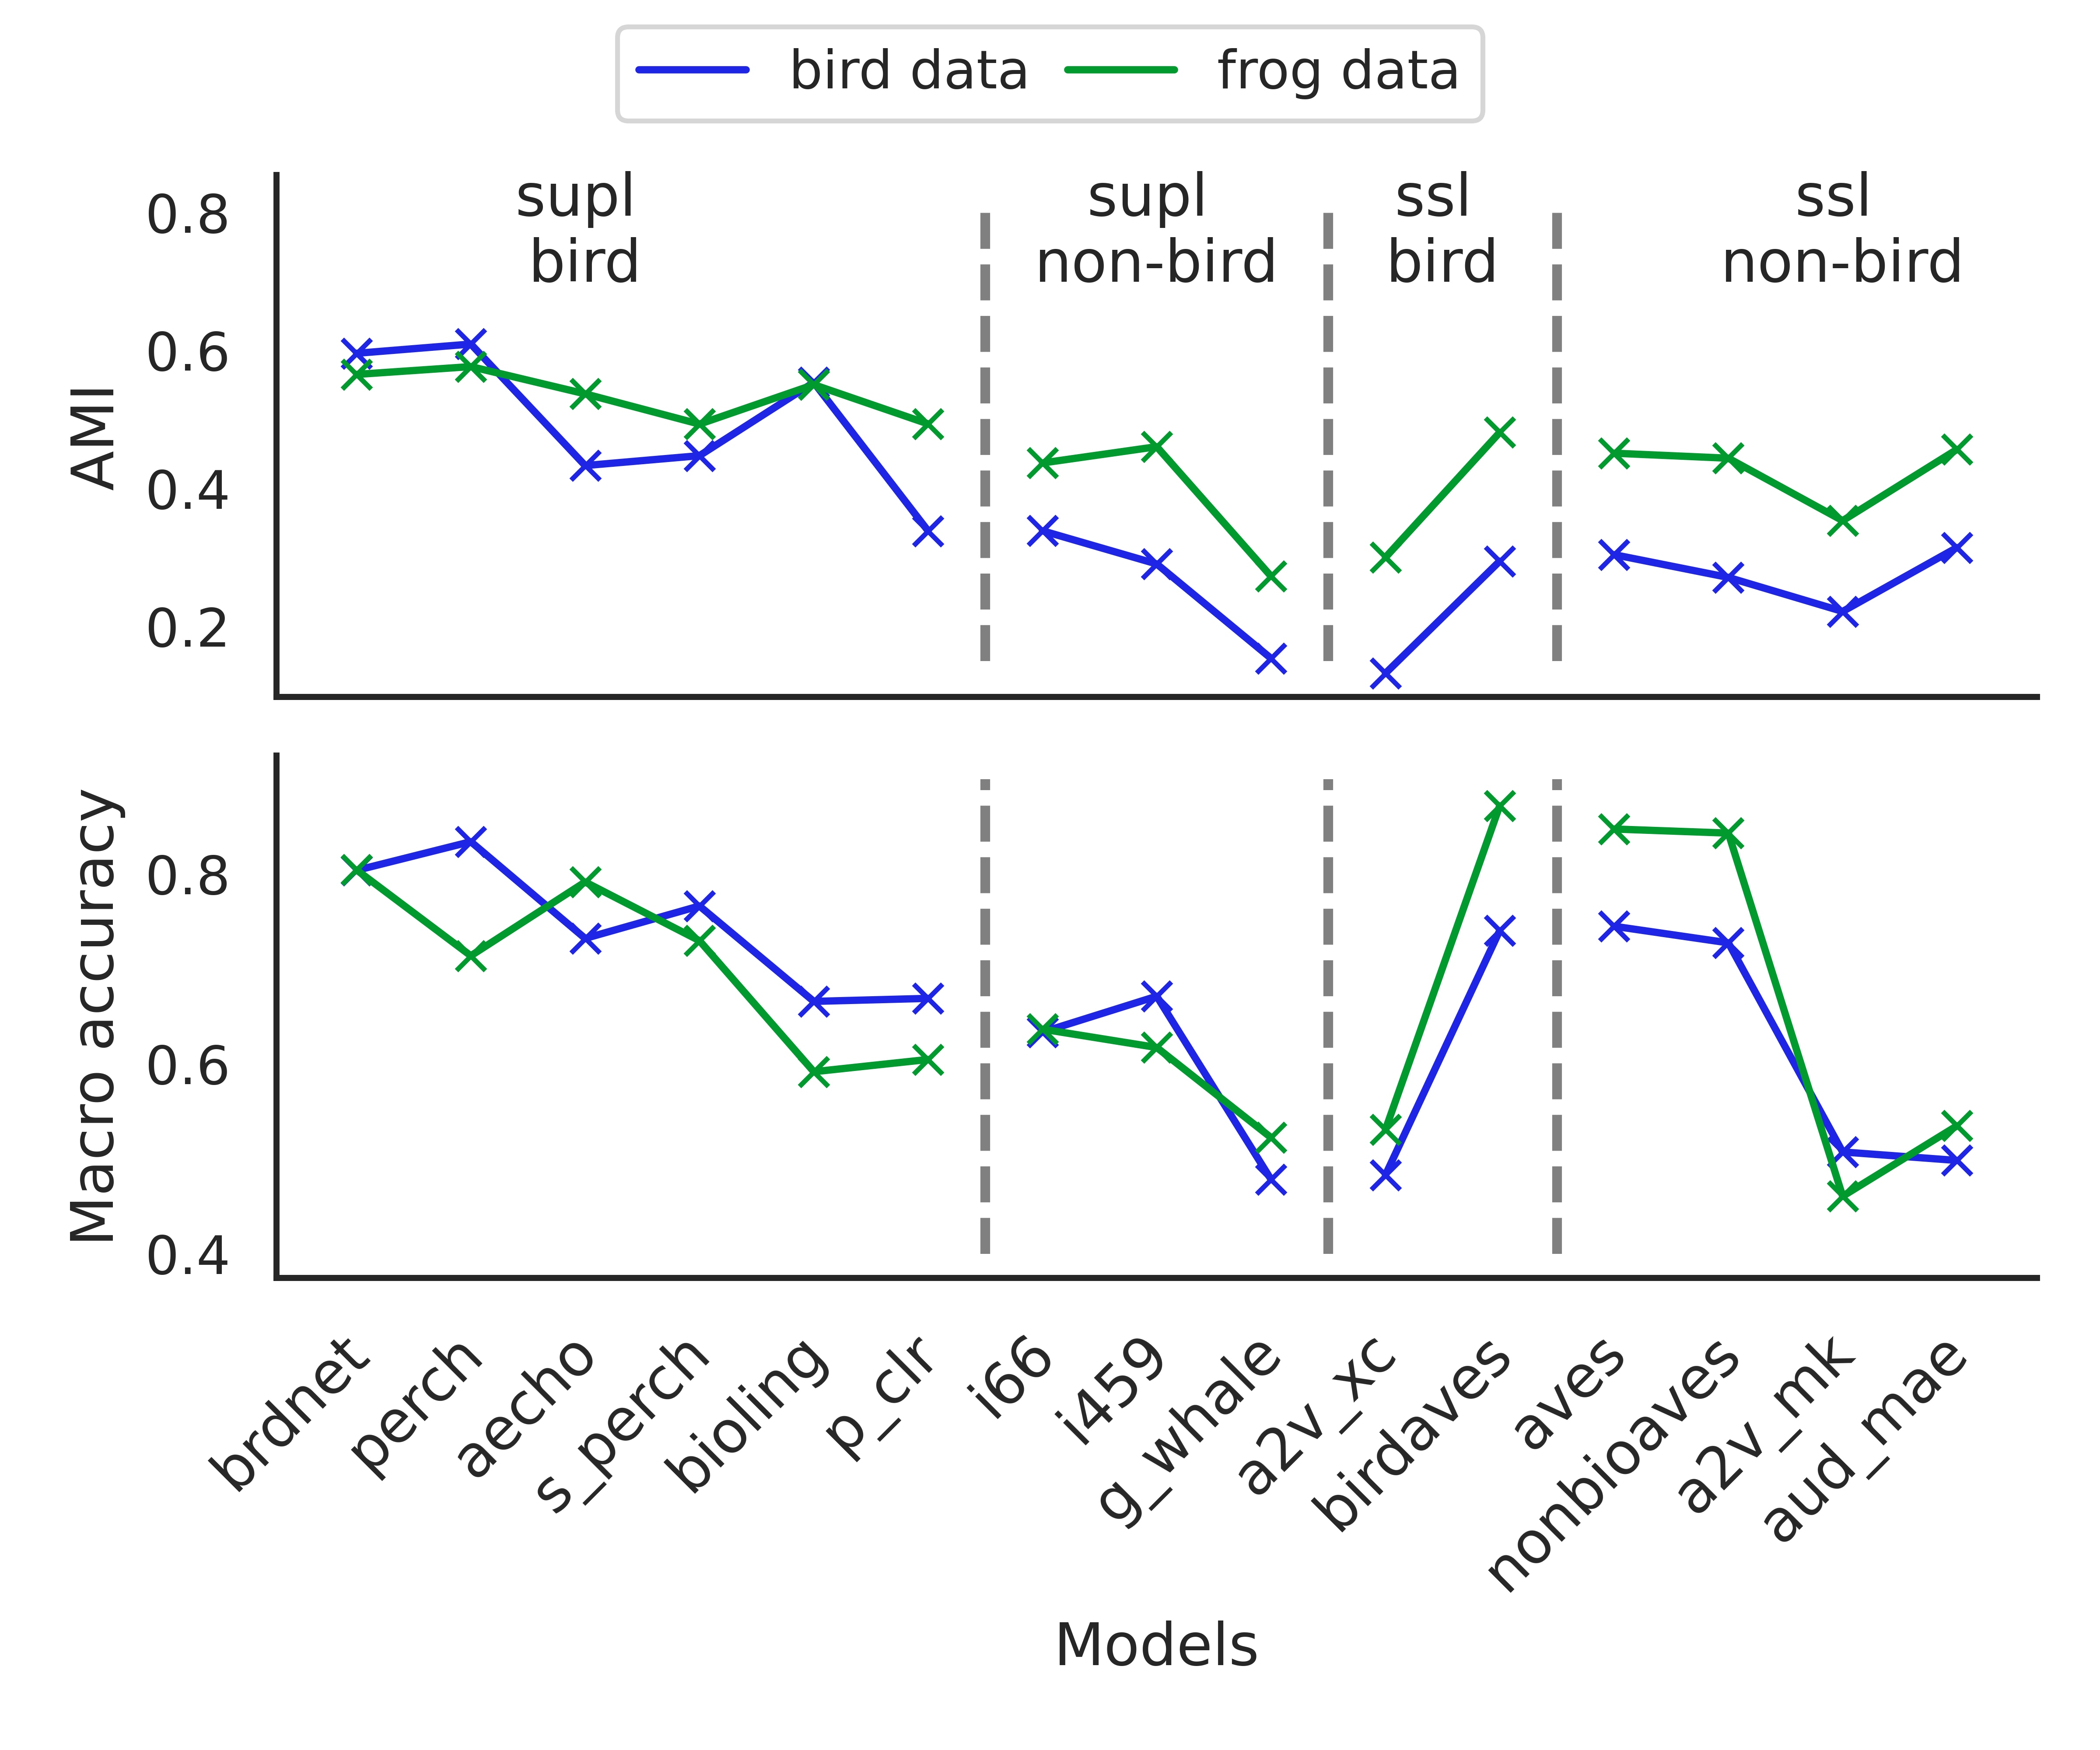
\includegraphics[width=8.1cm]{Sections/imgs/clust_and_class_lineplots.png}}}
    \caption{Comparison of feature extractor performance by learning paradigm, training data and application data. 
    The top plot shows clustering results of AMI.
    The bottom plot shows macro accuracy results of kNN classification. 
    Colors correspond to performance of the feature extractors when applied to bird data (blue) and frog data (green).
    The x-axis shows abbreviated model names, corresponding to abbrev. column in Tab.~\ref{tab:bacpipe_models}. 
    Models are grouped into categories along the x-axis by training paradigm (supervised learning (supl) and self-supervised learning (ssl)) and training data (bird data and non-bird data, see Table~\ref{tab:bacpipe_models}.}
    \label{fig:orig_vs_ump}
\end{figure}

In green we can see the performance when the feature extractors are applied to the frog data.
Among supervised learning feature extractors, changes in both clustering and kNN classification performance are varied.
Especially the three best performing models by clustering for the bird data, Perch, BirdNET and Biolingual, all decrease in performance when applied to the frog dataset.
The non-bird trained supervised learning feature extractors (supl non-bird) all improve their clustering performance by a large margin.
All self-supervised feature extractors vastly improve in clustering performance and aside from Animal2vec\_MK also in kNN classification.
The self-supervised AVES feature extractors (BirdAVES, AVES and NonBioAVES) drastically improve in both clustering and kNN classification on the frog data.
So much so, that all three outperform all other feature extractors by kNN classification.
% Aside from all feature extractors increase in clustering performance.

All non-bird trained feature extractors improve in clustering when applied to frog data.
Again, when applied to the frog dataset, all bird trained feature extractors except for Animal2vec\_XC outperform the rest by clustering and the top 6 models are the supervised learning bird trained feature extractors.
Among them, only AvesEcho improves in both clustering and kNN classification.
However, by kNN classification, results are more mixed by both training paradigm and training domain.

% When referring back to Table \ref{tab:bacpipe_models} embedding dimension does not correlate with clustering or kNN classification performance.
% Furthermore, the only two feature extractors trained on marine sounds, Google\_Whale and SurfPerch (trained on birds and marine sounds) reach very different performances.

For a more qualitative analysis of the different embedding spaces, two-dimensional UMAP embeddings of the feature extractors applied to the bird data are shown in Fig.~\ref{fig:embeds}.
The worst performing feature extractors, produce large unstructured clouds of mixed color, indicating that no significant clustering is achieved.
In the first and second row, feature extractors can be seen to separate the embeddings into meaningful clusters.
It is noticeable that some feature extractors such as AvesEcho\_PaSST and ProtoCLR seem to generate more subclusters than most other feature extractors.
This, however does not reflect in their performance in Fig.~\ref{fig:orig_vs_ump}.
The seven best performing feature extractors are all trained using supervised learning and the top three are additionally trained on bird vocalizations.
All three of the AVES models (BirdAVES, AVES and NonBioAVES) reach similar performances in spite of big differences in their fine-tuning datasets \cite{hagiwara_aves_2022}.
Despite the embedding spaces of BirdAVES and Animal2vec\_XC looking similarly cluttered, their performance varies by clustering and even more so my classification (see Fig.~\ref{fig:orig_vs_ump}).


\begin{figure*}[ht]
    \centerline{{
    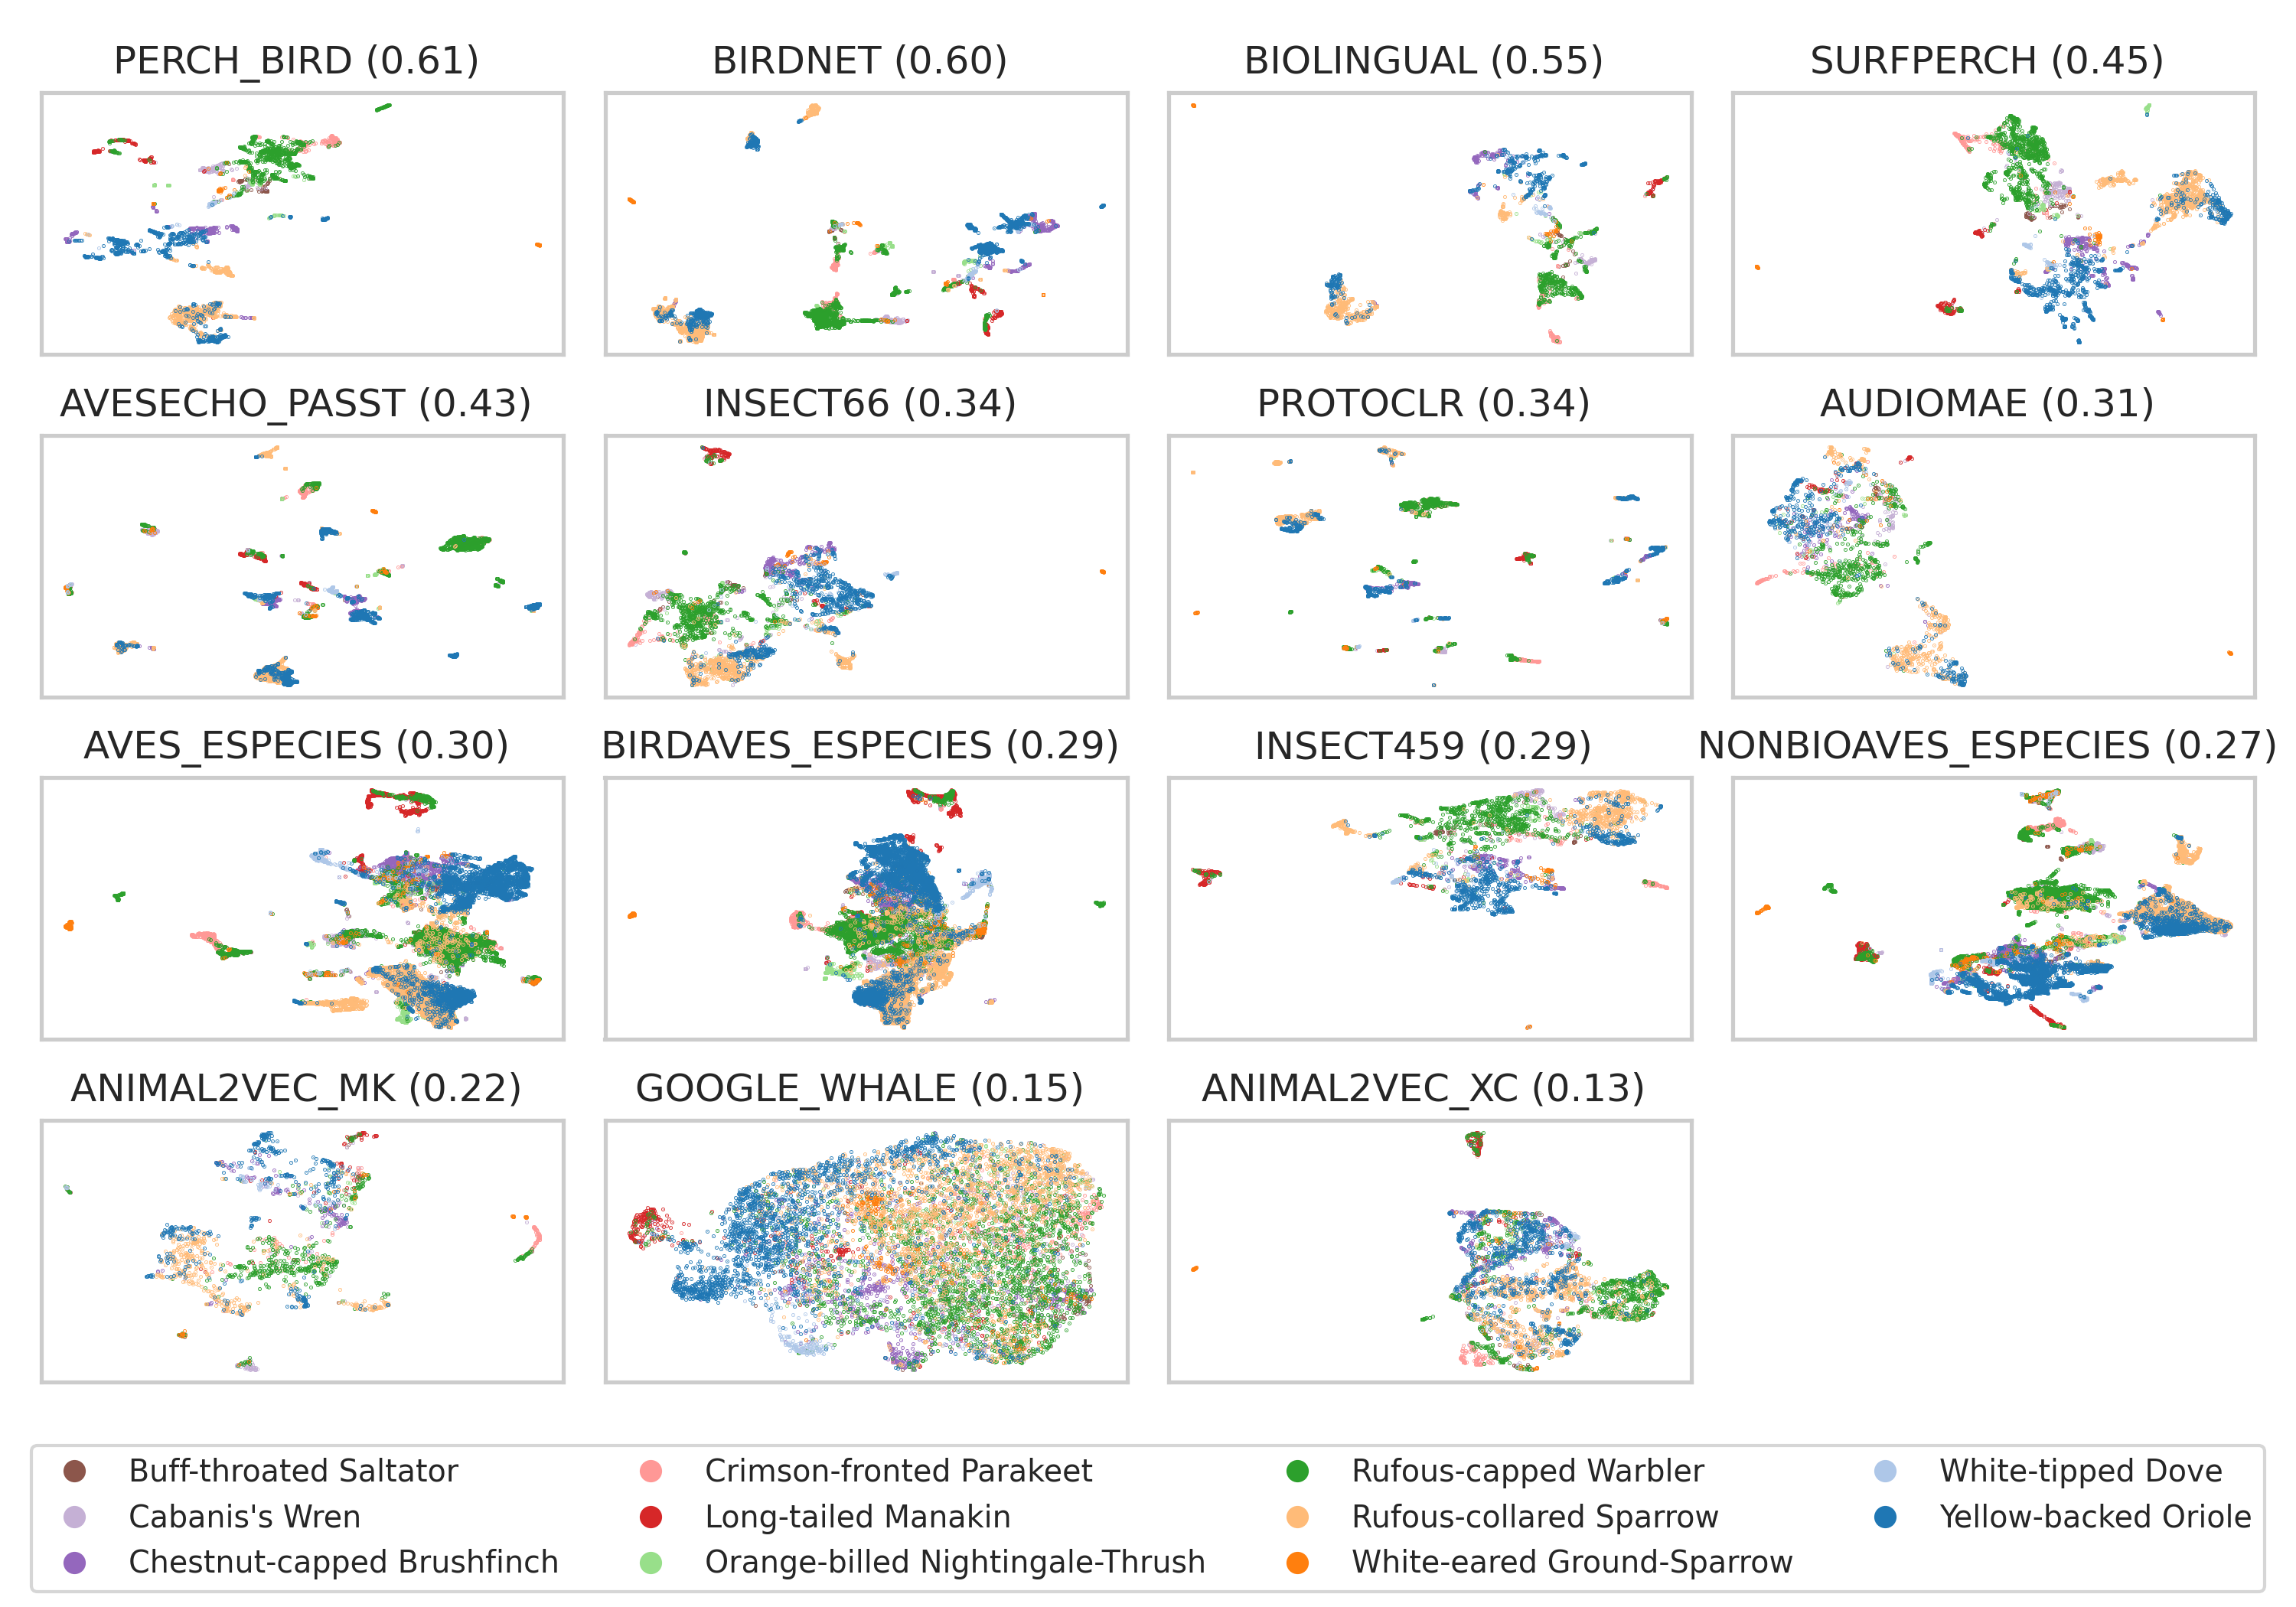
\includegraphics[width=16.3cm]{Sections/imgs/normal_overview.png}}}
    \caption{Two-dimensional embedding spaces of all feature extractors applied to bird data, sorted descending by their clustering performance of AMI values (indicated next to their name) from top left to bottom right.
    % Given the different input lengths of the feature extractors, the number of embeddings vary significantly.
    Colors correspond to the class labels, which are 11 different tropical bird species.}
    \label{fig:embeds}
\end{figure*}